%
% teil3.tex -- Beispiel-File für Teil 3
%
% (c) 2020 Prof Dr Andreas Müller, Hochschule Rapperswil
%
% !TEX root = ../../buch.tex
% !TEX encoding = UTF-8
%
\section{Die komplexe Schallintensität
\label{helmholtz:section:Schallintensitaet}}
\kopfrechts{Die komplexe Schallintensität}

\subsection{Definition und Bedeutung der komplexen Schallintensität
\label{helmholtz:subsection:def_Schallintensitaet}}

Die komplexe Schallintensität $\mathbf{I}_c$ erweitert das Konzept der Schallintensität und erlaubt eine umfassendere Analyse des akustischen Energieflusses. Sie ist definiert als:

\begin{equation}
\mathbf{I}_c (\mathbf{r}) = \frac{1}{2} \: p(\mathbf{r}) \: \mathbf{u}^{*}(\mathbf{r}),
\label{helmholtz:equationIntensitaetKomplex}
\end{equation}

\noindent wobei $p(\mathbf{r})$ den komplexen Schalldruck und $\mathbf{u}^{*}(\mathbf{r})$ die komplexe Konjugation der Partikelgeschwindigkeit $\mathbf{u}(\mathbf{r})$ beschreibt. Diese Formulierung berücksichtigt die Phasenverschiebung zwischen Schalldruck und Schallgeschwindigkeit und ermöglicht die Zerlegung des Energieflusses in quellenfreie und wirbelfreie Anteile gemäss der Helmholtz-Zerlegung.

Alternativ kann die komplexe Schallintensität auch wie folgt geschrieben werden:

\begin{equation}
\mathbf{I}_c (\mathbf{r}) = \underbrace{\mathbf{I}(\mathbf{r})}_{\frac{1}{2} \operatorname{Re} \, \{ p(\mathbf{r}) \, \mathbf{u}^*(\mathbf{r}) \}} + \underbrace{j\,\mathbf{Q}(\mathbf{r})}_{\frac{1}{2} \operatorname{Im} \, \{ p(\mathbf{r}) \, \mathbf{u}^*(\mathbf{r}) \}},
\label{helmholtz:equationIntensitaetKomplex_2}
\end{equation}  

\noindent wobei $\mathbf{I}(\mathbf{r})$ die aktive Intensität und $\mathbf{Q}(\mathbf{r})$ die reaktive Intensität darstellen. Diese beiden Komponenten haben unterschiedliche physikalische Bedeutungen, die im Folgenden näher erläutert werden.

\subsection{Eigenschaften der Intensitätskomponenten
\label{helmholtz:subsection:def_Schallintensitaet}}

Die beiden Komponenten der komplexen Schallintensität haben unterschiedliche physikalische Eigenschaften und Bedeutungen:

\begin{itemize}
\item Die \textbf{aktive Intensität} $\mathbf{I}(\mathbf{r})$ (Realteil) beschreibt den zeitgemittelten Netto-Energiefluss pro Fläche an dem Ort $\mathbf{r}$ und lässt sich ausdrücken als:
\begin{equation}
\mathbf{I}(\mathbf{r}) = \frac{1}{T}\int_0^T \mathbf{I}_i(\mathbf{r},t)\,\mathrm{d}t = \frac{1}{2}\Re\{p(\mathbf{r})~\mathbf{u}^*(\mathbf{r})\}.
\end{equation}

\noindent In quellenfreien, stationären Feldern ohne Energieabsorption gilt:
\begin{equation}
\nabla \cdot \mathbf{I} = 0.
\end{equation}

\item Die \textbf{reaktive Intensität} $\mathbf{Q}(\mathbf{r})$ (Imaginärteil) beschreibt die zeitlich gemittelte Dichte der nicht-propagierenden, oszillierenden Energie: 
\begin{equation}
\mathbf{Q}(\mathbf{r}) = \frac{1}{2}\Im\{p(\mathbf{r})~\mathbf{u}^*(\mathbf{r})\}.
\label{helmholtz:equationReaktiveIntensitaet}
\end{equation}

\noindent Sie ist wirbelfrei:
\begin{equation}
\nabla \times \mathbf{Q} = 0
\end{equation}

\noindent Und steht in direkter Beziehung zur Differenz zwischen kinetischer Energie (T) und potentieller Energie (V):
\begin{equation}
\nabla \cdot \mathbf{Q} = -2 \omega [T-V]
\end{equation}
\end{itemize}


\subsection{Mathematische Analyse der Intensitätskomponenten
\label{helmholtz:subsection:def_Schallintensitaet}}

Die mathematische Analyse der Intensitätskomponenten liefert wichtige Einsichten in die Struktur des akustischen Feldes. Besonders aufschlussreich ist die Untersuchung der Divergenz und Rotation dieser Vektorfelder.

\subsubsection{Divergenz der aktiven Intensität}

Die Divergenz der aktiven Intensität beschreibt Quellen und Senken im Energiefluss:

\begin{equation}
\nabla \cdot \mathbf{I} = -\omega\text{Im}\{p^*q\} - \alpha|p|^2,
\end{equation}

\noindent wobei $q$ die Volumengeschwindigkeit der Schallquelle und $\alpha$ der Absorptionskoeffizient des Mediums ist. Diese Gleichung repräsentiert eine Energiebilanz: Quellen erzeugen Energie ($q$), und Absorption verringert sie ($\alpha$).

In quellenfreien, verlustfreien Gebieten gilt:

\begin{equation}
\nabla \cdot \mathbf{I} = 0,
\end{equation}

\noindent was bedeutet, dass keine Energie erzeugt oder vernichtet wird, sondern nur fließt.

\subsubsection{Rotation der aktiven Intensität}

Die Rotation der aktiven Intensität ist nicht notwendigerweise null und kann geschrieben werden als:

\begin{equation}
\nabla \times \mathbf{I} = \frac{k}{c} \frac{\mathbf{I} \times \mathbf{Q}}{V},
\end{equation}

\noindent wobei $k$ die Wellenzahl, $c$ die Schallgeschwindigkeit und $V$ die potentielle Energie des Feldes ist. Dies zeigt, dass Wirbelstrukturen in der aktiven Intensität auftreten können, wenn aktive und reaktive Intensität nicht parallel sind.

\subsubsection{Divergenz der reaktiven Intensität}

Die Divergenz der reaktiven Intensität ist verbunden mit der Energieverteilung zwischen kinetischer und potentieller Form:

\begin{equation}
\nabla \cdot \mathbf{Q} = -2 \omega [T-V],
\end{equation}

\noindent wobei $T$ die kinetische und $V$ die potentielle Energiedichte sind. Positive Divergenz bedeutet, dass mehr kinetische als potentielle Energie vorhanden ist, während negative Divergenz das Gegenteil impliziert.

\subsubsection{Rotation der reaktiven Intensität}

Die reaktive Intensität ist immer wirbelfrei:

\begin{equation}
\nabla \times \mathbf{Q} = 0,
\end{equation}

\noindent was bedeutet, dass sie als Gradient eines skalaren Potentials darstellbar ist. Dies ist eine fundamentale Eigenschaft, die eine direkte Verbindung zur Helmholtz-Zerlegung herstellt, wie im nächsten Kapitel näher erläutert wird.

\subsubsection{Wirbelstrukturen und Quellen}

Die mathematische Analyse zeigt, dass aktive und reaktive Intensitätsfelder charakteristische Quellen-, Senken- und Wirbelstrukturen aufweisen können, wie in Abbildung \ref{fig:Schallintensitaet} dargestellt.

\begin{figure}[h!]
\centering
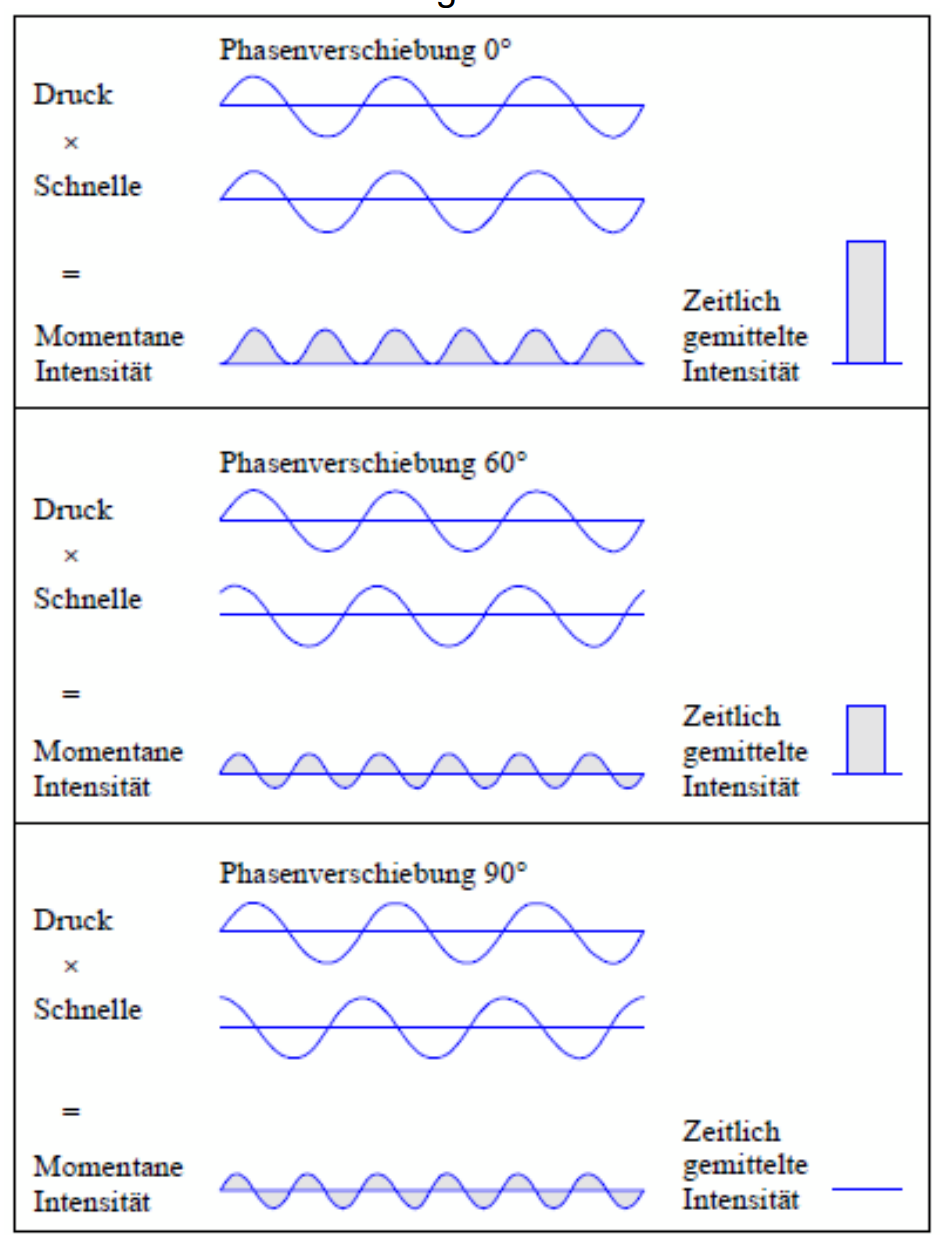
\includegraphics[scale=0.4]{papers/helmholtz/images/Schallintensitaet.png}
\caption{Schematische Darstellung der Quellen- und Wirbelstrukturen in einem Schallintensitätsfeld}
\label{fig:Schallintensitaet}
\end{figure}

Diese Strukturen sind von großer Bedeutung für die Schallquellenidentifikation und die Analyse von Energieflüssen in akustischen Feldern. Die Verbindung zwischen diesen Strukturen und der Helmholtz-Zerlegung wird im folgenden Kapitel näher betrachtet.




